\section{Репликоны.
Инициация раунда репликации ДНК Escherichia coli. Белки участвующие в регуляции инициации 
репликации (DnaABC, ssb, SeqA, dam).
Топологические проблемы репликации. Сегрегация репликонов по бактериальным клеткам.
Репликация плазмид, мобильных элементов, фагов и вирусов.
Особенности репликации в эукариотах. Теломеры и центромеры. Сегрегация хромосом.}

\subsection{Репликоны}

\textbf{Репликон} — молекула или участок ДНК или РНК, реплицирующийся из одного места начала репликации.

Задача: реплицировать ДНК. 

Как ее можно решать: посадить белки в одном месте и проехаться ими по всей ДНК (бактерии) или распараллелить процесс, посадив много белков в разных местах (эукариоты).

Например, у прокариот кольцевая ДНК имеет одну точку начала репликации, таким образом, она вся - репликон (см. рис. \ref{fig:6_replicon2}). У эукариот длинная линейная ДНК имеет множество точек начала репликации, то есть у нее много репликонов (см. рис. \ref{fig:6_replicon2}, \ref{6_replicon1}).

\begin{figure}[h!]
    \centering
    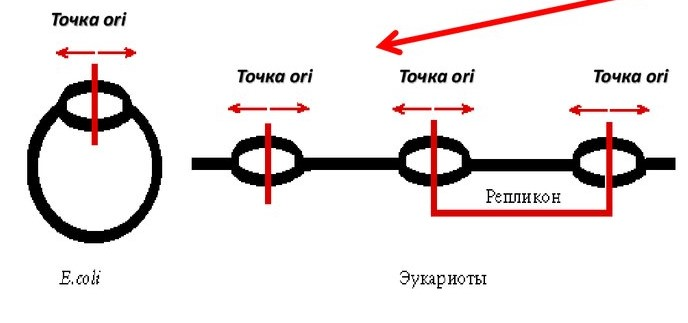
\includegraphics{6_replicon2.jpg}
    \caption{Иллюстрация репликонов бактерий и эукариотов. Слева - кольцевая ДНК кишечной палочки, у нее одно место начала (ori) репликации и она сама один репликон. Саправа - линейная ДНК эукариот со множеством репликонов. Стрелочками обозначены движения репликационных вилок.}
    \label{fig:6_replicon2}
\end{figure}

\begin{figure}
    \centering
    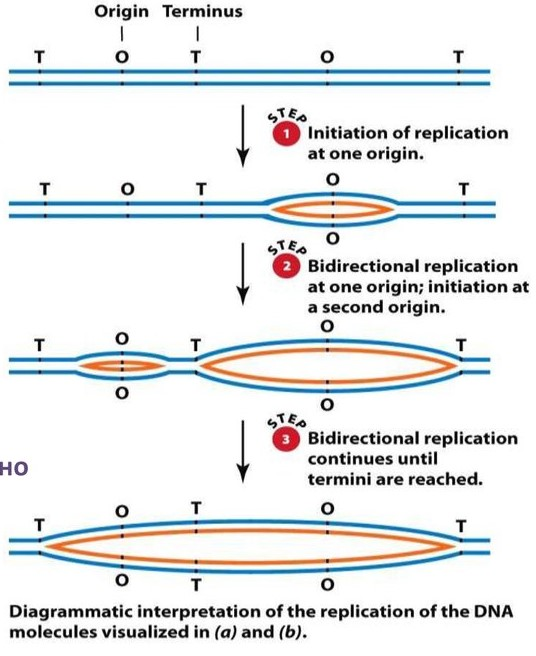
\includegraphics[width = 0.5 \linewidth]{6_replicon1.jpg}
    \caption{Репликоны эукариот - участки от O (origin) до T (termini).}
    \label{fig:6_replicon1}
\end{figure}

\subsection{Инициация раунда репликации ДНК Escherichia coli. Белки участвующие в регуляции инициации 
репликации (DnaABC, ssb, SeqA, dam).}

Здесь мы рассмотрим подробно процесс запуска репликации ДНК кишечной палочки с перечислением некоторых конкретных белков. (Подробнее о репликации см. билет 3.)

Имеется кольцевая двухцепочечная молекула ДНК со специальной точкой (читай, местом) начала репликации OriC. Клетка набрала достаточную массу для начала деления. 

\begin{itemize}
    \item Белки dnaA узнают OriC, садятся на ДНК и начинают раскручивать его. То есть, если смотреть на принципиальную схему репликации (билет 3, рис. \ref{fig3:rep}), dnaA является топоизомеразой кишечной палочки.
    
    \item Белок dnaC помогает белку dnaB сесть на ДНК и начать его разделять на две несвязанные цепи в том месте, где его расплела dnaA. Таким образом, dnaB - хеликаза кишечной палочки.
    
    \item SSB-белки удерживают две цепи ДНК, разделенные dnaB, от обратного связывания друг с другом.
    
    \item SeqA - белок, который садится на ДНК в области oriC после инициации репликации и не подпускает остальные белки для повторной инициации (потому что задача синтезировать две двухцепочечные молекулы ДНК из одной и распределить их по дочерним клеткам, а не размножать ДНК в геометрической прогрессии, пока у клетки не кончатся ресурсы).
    
    \item Dam - приходит на место посадки SeqA и <<обрабатывает>> (метилирует аденин) новые дочерние цепи ДНК так, чтобы на них dnaA не садилась уже по умолчанию (до тех пор, пока дочерняя клетка не вырастет), а не только пока их область OriC закрыт белками SeqA.
\end{itemize}

\subsection{Топологические проблемы репликации.}

При удвоении кольцевой ДНК бактерий могут получиться два кольца, сцепленных друг с другом (см. рис. \ref{fig:6_topology}). Их разделение производит топоизомераза II, или гираза. Она делает разрыв, через который проводит двухцепочечную нить ДНК, и снова сшивает.

\begin{figure}[h!]
    \centering
    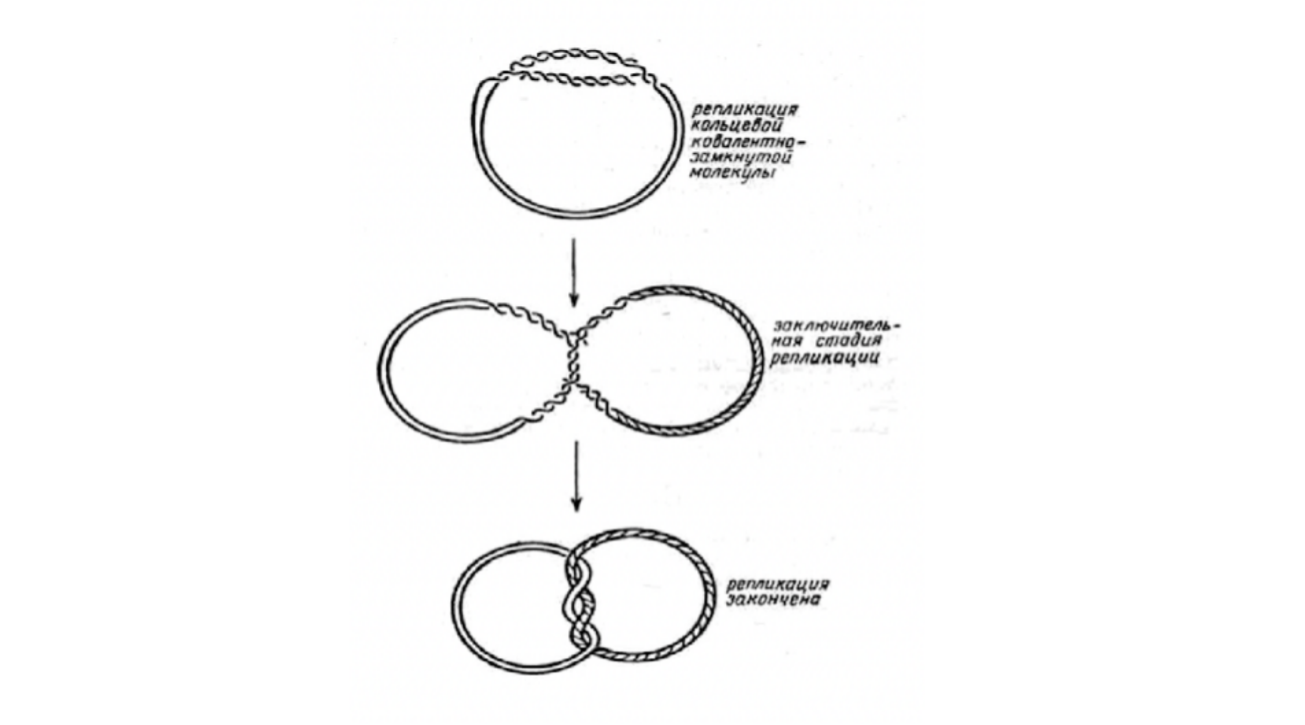
\includegraphics[width = 0.8 \linewidth]{6_topology.png}
    \caption{Топологические проблемы репликации кольцевых молекул ДНК (на две материнских цепи ДНК в кольце тоже переплетены ирл, просто для упрощения восприятия их так нарисовали).}
    \label{fig:6_topology}
\end{figure}

\subsection{Сегрегация репликонов по бактериальным клеткам.}

Прокариоты, в отличие от эукариот, не имеют такого сложного механизма деления клетки (см. билет про метоз и мейоз и сравнить с картинкой \ref{fig:6_deleniye}). Например, у них не образуется стадии <<веретена>>. Конкретный механизм сегрегации хромосом (одна хромосома у прокариот является также репликоном, см. параграф выше) не описан. 

\begin{figure}[h!]
    \centering
    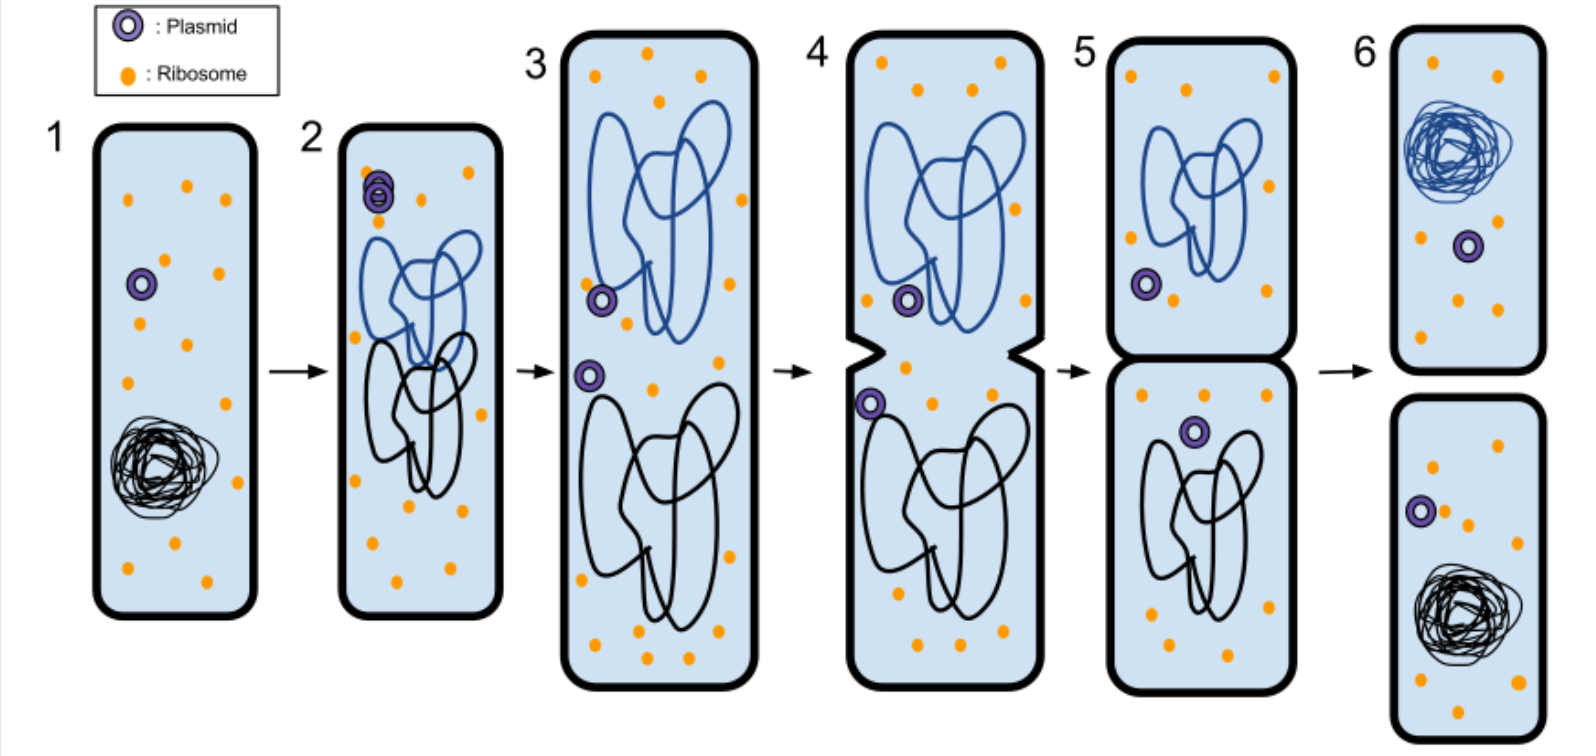
\includegraphics[width = 0.7 \linewidth]{6_deleniye.png}
    \caption{Деление бактериальной клетки: 1)  начальное состояние, 2) репликация ДНК, 3) сегрегация хромосом по клеткам, 4-5) образование перегородки между клетками, 6) финал, две клетки.}
    \label{fig:6_deleniye}
\end{figure}

\subsection{Репликация плазмид, мобильных элементов, фагов и вирусов.}

\begin{itemize}
    \item \textbf{Плазмиды} - небольшие кольцевые молекулы ДНК бактерий, физически обособленные от хромосом и способные к автономной репликации (то есть, вне стадии деления клетки). Они реплицируются по двум схемам: по типу катящегося колеса и по тета-типу (см. билет 3).
    
    \item \textbf{Мобильные генетические элементы} - куски генетического материала, которые могут путешествовать внутри генома и от одного организма к другому (буквально цепочки нуклеиновых кислот, отсоединяющиеся от хромосом в одном месте, диффундирующие, и встраивающиеся в другом)
    
    \item \textbf{Вирусы} - неклеточный инфекционный агент, который может воспроизводиться только внутри клеток. Вирус фактически представляет собой небольшую белковую машину и генетический материал.
    
    Вирус проникает в организм хозяина. Затем вирус прикрепляется к мембране клетки, специальными белками буравит клеточную мембрану и впускает внутрь свой генетический материал. Белки клетки начинают реплицировать генетический материал вируса и на его основе собирать белки, из которых получаются новые вирусы. 
    
    Когда все ресурсы клетки израсходованы, разможившиеся копии вируса разрывает клетку и высвобождаются для заражения новых клеток.
    
    \item \textbf{Бактериофаги} - вирусы, поражающие бактерии. К ним справедливо все то же самое, что изложено про вирусы.
    
\end{itemize}

\subsection{Особенности репликации в эукариотах. Теломеры и центромеры. Сегрегация хромосом.}

У эукариот молекулы ДНК линейны. Рассмотрим обычную (не половую, важно) клетку эукариот. 

\begin{itemize}
    \item Всю жизнь от рождения от материнской клетки дочерняя клетка живет с хромосомами. Хромосомы - длинные нити ДНК, на которых в некоторых местах еще сидят структурные белки. Число типов хромосом и число копий одного типа варьируется от вида к виду.
    
    \item Перед делением клетки ДНК хромосомы реплицируются и из одной материнской хромосомы получается две дочерние, называющиеся \textbf{сестринскими хроматидами} (см. рис. \ref{fig:6_chromatide}).
    
    \begin{figure}[h!]
        \centering
        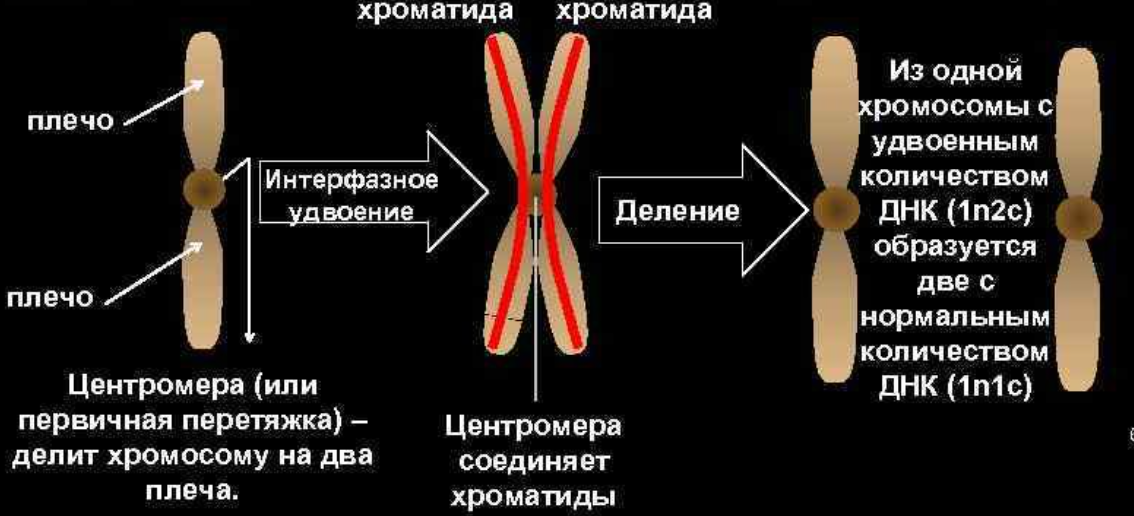
\includegraphics[width = 0.7 \linewidth]{6_chromatide.png}
        \caption{Хроматиды и хромосомы}
        \label{fig:6_chromatide}
    \end{figure}
    
    \item Хроматиды связаны белками в некоторой области. Эта область называется \textbf{центромера} (рис. \ref{fig:6_chromosome}).
    
    \item Концевые участки хромосом называются \textbf{теломеры}.
    
    \begin{figure}[h!]
        \centering
        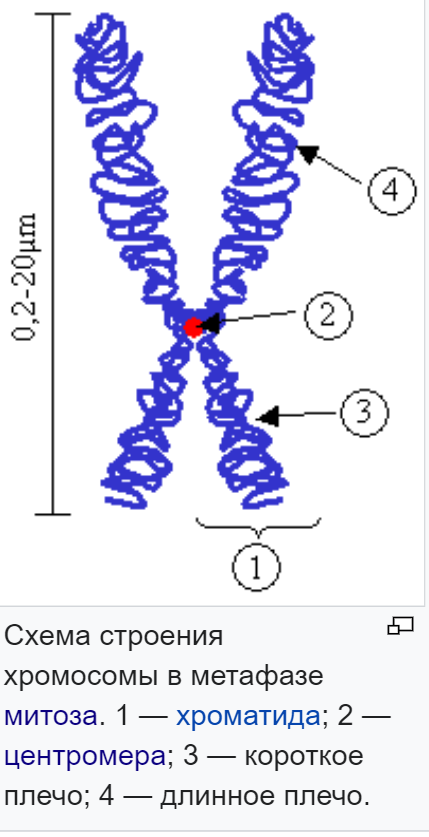
\includegraphics{6_chromosome.png}
        \caption{Хромосома, состоящая из двух хроматид}
        \label{fig:6_chromosome}
    \end{figure}
    
    \item В процессе клеточного деления происходит \textbf{сегрегация хромосом}. Каждой из двух дочерних клеток переходит одна из сестринских хроматид (см. подробнее митоз и мейоз). А ОКАЗАВШИСЬ В ДОЧЕРНЕЙ КЛЕТКЕ ХРОМАТИДЫ УЖЕ НАЗЫВАЮТСЯ СНОВА ХРОМОСОМАМИ НЕНАВИЖУ ОБОЗНАЧЕНИЯ БИОЛОГОВ
\end{itemize}
